\section{Extracting character metadata} \label{sec:metadata}
Our metadata predicting model builds on two hypotheses about where in a work of fiction a character's metadata (job, gender, family, etc.) can be explicitly found. In literary terms, this metadata can be considered part of a \textit{characterization}. 

For a given character $c_i$, we posit the following (notation explained below):
\begin{enumerate}
\item explicit elements of $c_i$'s metadata are likely to be within a window $w$ surrounding an occurrence of $c_i$
\item explicit characterization is more likely to occur within the first $k$ occurrences of $c_i$
\item explicit characterization is more likely in a sentence where $c_i$, but no $c_j \in \mathcal{C}$ occurs, $i \neq j$.
\end{enumerate}

In section 5 we discuss how our predictors support these hypotheses.

For a given book, we define a character $c_i$, such that $c_i \in \mathcal{C}$, where $\mathcal{C}$ is a set of size $N$. Each book is split into sentences $s_j \in \mathcal{S}$, $\mathcal{S}$ of size $M$ (number of sentences in book). 

The term \textit{window} in hypothesis 1. describes a batch of either words or sentences, taken before and after a character occurrence. So for a given window wing size $w$, and the $k$th occurrence over the whole book of $c_i \in \mathcal{C}$  in sentence $s_j$, we have a window $W_{\mu^i_k}$, s.t. 

\begin{equation}
W_{\mu^i_k} = [s_{j-w}, s_{j-w+1}, ...,  s_{j-1}, s_{j}, s_{j+1}, ..., s_{j+w-1}, s_{j+w}]
\end{equation}

where $\mu^i_k$ is the $k$th occurrence of $c_i$, and $0 \leq k \leq L_i$, so $c_i$ has a total of $L_i$ occurrences in the book. In this way, a window is of size $2w + 1$. Note that the inferior and superior bounds for a window are $s_0$ and $s_m$, so the leftmost sentence in any case is actually $s_{\min(0, j-w)}$, and the rightmost $s_{\max(m, j+w)}$. An example is given for character \textit{Phileas Fogg} in \cref{fig:window}

\begin{figure}
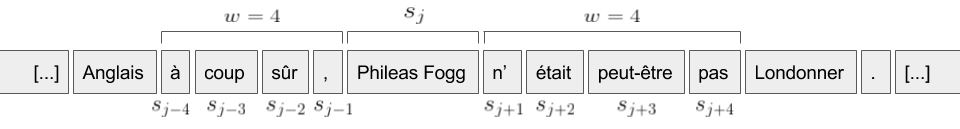
\includegraphics[width=\textwidth]{fig/window.png}
\caption{Window example, with w=4. Note, in  this sentence all tokens are taken for consideration, whereas in practice we worked with sentences without stopwords, and more in some cases (e.g. only specific PoS tags). We also use words to determine the window. In practice, this could also be whole sentences instead.}
\label{fig:window}
\end{figure}

For character $c_i$, let its document $D^{c_i}$ be the collection of all the windows with an occurrence of $c_i$ at their center. This whole description can be taken analogously for windows of words instead of sentences. We experimented with different window parameters for the various predictors described below. 

\vspace*{1em}
% Hypothesis 2
Hypothesis 2 implies that metadata is more likely to be found in the initial $\mu^i_k$. This is verified in the predictors by comparing different methods. We decided on two representations of this. A natural first possibility is to constrain $D^{c_i}$ to the first $k$ occurrences of $c_i$. We write this $D^{c_i}_{[0:k]}$. 

Additionally, we used weights $\omega^i_k$ for a mention $k$ of $c_i$ that decrease as $k$ increases. For this purpose, an exponentially decreasing function was chosen, such that if we want to compute the weight $\omega$ for a measure for a given predictor of $c_i$ at mention $k$, we have
\begin{equation}
\omega^i_k = -\log (\frac{k+1}{L_i})
\end{equation}


% Hypothesis 3
Hypothesis 3 stipulates that if $c_i$ occurs without the mention of any other characters in the book, then explicit characterization is more likely, or at least, some shallow techniques might be more precise. We test this by using a filtered document 
\begin{equation}
D^{c_i}_{filt} = D^{c_i} \backslash \bigcup_j D^{c_j}
\end{equation}
where $i \neq j$. 

Of course the hypotheses discussed are not conflicting in nature and can be applied alongside each other, and were tested as such for our predictors. With this setup, we went on to try different approaches to extracting metadata for individual or a whole collection of characters in a book.

\subsection{Extraction by LDA}
As a preliminary exploration of the characterization of an entity in a book, we applied a latent dirichlet allocation (LDA) \cite{blei2003latent} on the document of the entity. By this generative probabilistic model, we get a requested amount of topics, each topic being a distribution over the words of the document. The implementation discussed below can be found in the \texttt{LDACapture.py} file.

Since this is basically an unsupervised way of extracting data, we get results that are not specifically pertinent to characterization, but more a broad indicator of the whole narrative (local to the given character). However, some of the topics were found to be pertinent. This is mainly in cases where the metadata considered plays a recurrent and central part in the narrative.

To extract them, we first focused on a particular aspect we wanted to observe. For instance, the model is more likely to capture information about a profession if it is provided only with common and proper nouns, since this filters out 'noise' irrelevant to this question (adverbs, adjectives, etc... verbs could be indicative, but there are many more generic ones that have a higher probability within any standard text). This filtering is achieved with the probabilistic tagging provided by TreeTagger. Additionally, we work exclusively with lemmas (also, provided by TreeTagger), when they are known, in order to minimize morphological variations.

If we take an example from \textit{Au Bonheur des Dames}, and look at the topics generated for the main character Denise, a saleswoman in a clothing store, by providing the LDA model with sentences containing only occurrences of the token `Denise', it's obvious that the concept of shops is indicated (words like \textit{magasin}, \textit{boutique}, \textit{vêtement}, \textit{rayon}.

\begin{lstlisting}
Topic 0 - 0.083*"magasin" + 0.055*"dames" + 0.055*"bonheur" + 0.055*"émotion" + 0.042*"question" + 0.042*"larme" + 0.028*"air" + 0.028*"heure" + 0.028*"idée" + 0.028*"vérité"

Topic 1 - 0.054*"boutique" + 0.054*"place" + 0.054*"bouche" + 0.054*"oncle" + 0.054*"tour" + 0.037*"cœur" + 0.037*"moi|mois" + 0.037*"œil" + 0.037*"peur" + 0.037*"silence"

Topic 2 - 0.066*"peur" + 0.050*"elle-" + 0.050*"fraîcheur" + 0.034*"œil" + 0.034*"larme" + 0.034*"enfant" + 0.034*"famille" + 0.034*"vêtement" + 0.034*"geste" + 0.034*"désir"

Topic 3 - 0.091*"main" + 0.047*"oncle" + 0.047*"frère" + 0.047*"rayon" + 0.047*"chambre" + 0.047*"reste" + 0.047*"idée" + 0.024*"rue" + 0.024*"milieu" + 0.024*"dailleurs"
\end{lstlisting}

However, since this is a central theme of the whole book, it can't be seen as conclusive in any way. If we look instead at an example from \textit{Le tour du monde en quatre-vingt jours}, and take Passepartout, the valet, as the character, we get the following

\begin{lstlisting}
Topic 0 - 0.093*"pensée" + 0.071*"sac" + 0.071*"bank-notes" + 0.048*"jour" + 0.048*"maison" + 0.048*"brique" + 0.048*"esprit" + 0.048*"monsieur" + 0.025*"main" + 0.025*"train"

Topic 1 - 0.084*"train" + 0.067*"milieu" + 0.051*"maître" + 0.051*"livre" + 0.034*"jour" + 0.034*"pied" + 0.034*"chambre" + 0.034*"peine" + 0.034*"journée" + 0.034*"coup"

Topic 2 - 0.080*"heure" + 0.080*"rue" + 0.064*"maître" + 0.049*"ville" + 0.049*"exercice" + 0.049*"agent" + 0.033*"bord" + 0.033*"main" + 0.033*"montre" + 0.033*"yokohama"

Topic 3 - 0.248*"maître" + 0.059*"air" + 0.040*"paquebot" + 0.040*"hong-kong" + 0.040*"départ" + 0.040*"bord" + 0.040*"bonheur" + 0.021*"heure" + 0.021*"rangoon" + 0.021*"jusqu"
\end{lstlisting}

where the theme of travel is obviously dominant. Only weak indications of his profession can be found, in the word `ma\^itre' (master), recurring in several topics. 

After these disappointing results, we try the approach of writing specific predictors for metadata categories.

\subsection{Metadata-specific predictors}
We implemented three different predictors that focus on specific aspects of a character's metadata, i.e. profession, gender and sentiment. In this way we look at aspects from a character's \textit{activity}, \textit{person} and \textit{psychological affect}. In the implementations of these predictors, three different main methods are used that cover a good spread of conceivable additional predictors, i.e. ad-hoc lexicon-based and linguistic-rule-based, or using external tools.

The implementations discussed below can be found in the \texttt{computeMeta.py} file.

\subsubsection{Profession} \label{sssec:profession}
For predicting the profession of a character $c_i$, we utilized an external corpus \footnote{A list of approximately 2600 masculine and feminine profession titles at \href{http://www.vd.ch/guide-typo3/le-texte/rediger-pour-le-web/redaction-egalitaire/2000-noms-au-masculin-et-au-feminin}{http://www.vd.ch/guide-typo3/le-texte/rediger-pour-le-web/redaction-egalitaire/2000-noms-au-masculin-et-au-feminin}} of known professions in French. Let $p_k \in \mathcal{P}$ be the $k$th  profession in the list. 

Our approach is then split along two different measures. On the one hand, we look at the co-occurence \textbf{count}, i.e. 
\begin{equation}
count_{c_i, p_k} = \sum_j \mathbb{I}^{c_i}_j \mathbb{I}^{p_k}_j
\end{equation}
where the indicator functions $\mathbb{I}_j = 1$ if $c_i$ (resp. $p_k$) occurs in sentence (or window) $j$. This is computed $\forall c_i \in \mathcal{C}, \forall p_k \in \mathcal{P}$, and kept in a dictionary of $c_j \rightarrow [p_0, p_1, ...]$. The job with the highest count score is taken as the winner. 

On the other hand, we look at the mean \textbf{proximity} measure, so for given $c_i$ and $p_k$, get the mean distance between the two within a window. See \cref{alg:proximity} for a sketch of the implementation. 

\begin{algorithm} 
  \KwData{$charWindows, jobList, jobCount, char$}
  \KwResult{$score$}
  $score \leftarrow$ a map with jobs for keys and values $\leftarrow 0$\;
  \For{$win \in charWindows$}{
    \For{$job \in jobList$}{
      \If{$job \in win$}
      {$\texttt{increment}(jobCount[char], 1)$\;
      $dist = \texttt{abs}(\texttt{indexOf}(win, char), \texttt{indexOf}(win, job))$\;
      $\texttt{increment}(score[job], dist)$\;}                
    }
  }
  \For{$(job, value) \in score$}{
      $score[job] \leftarrow value / jobCount[job]$ 
  }
  \caption{Computing job proximity scores for a given character.}
  \label{alg:proximity}
\end{algorithm}

As before, this is computed $\forall c_i \in \mathcal{C}, \forall p_k \in \mathcal{P}$ and stored in a dictionary. The job with the lowest mean proximity score is taken as the winner.

Note, this gives an idea of the implementation for the count score as well, and can be applied to other aspects of a $c_i$'s metadata (e.g. family ties, nationality). The process needs a collection of keywords to extract from a given $D^{c_i}$, in the case of \cref{alg:proximity}, the \textit{jobList}, and a scheme for aggregating the occurrences into a score for each keyword, which is done here by the \textit{distance} function.

We additionally implemented an \textbf{aggregate predictor}, combining both proximity and count measures, where we add their weighted normalized scores together. The weights were chosen to approximate best results.


\subsubsection{Gender} \label{sssec:gender}
In order to predict the gender of a character, we tried to capture different lexical, linguistic and morphological aspects of a window surrounding that character. In turn, we captured the number of masculine and feminine pronouns in the window, the number of adjectives with feminine or masculine form, the number of obvious titles linked to the character. These scores were then combined to provide the best possible prediction.

\paragraph{Pronoun} We captured the masculine and feminine pronouns (`il', `elle') in the window containing $c_i$ (and for the words with the relevant PoS tag: \texttt{PRO:PER}), and aggregated the captures by adding $+1$ for each feminine, and $-1$ for each masculine occurrence. Note that this can be considered problematic due to the use of the masculine pronoun for the impersonal case as well (in english `it'), e.g. \textit{`il est clair que...'}. In practice, even with this strong assumption, the results weren't too biased towards predicting male characters.

\paragraph{Adjective} Lists of typical masculine and feminine adjective endings were compiled (e.g. \texttt{[`el', `er', `en', `on', ...]}, and \texttt{[`elle', `enne', `onne', `euse', ...]} respectively. For words with the relevant PoS tag (\texttt{ADJ}), we again aggregated these captures by a similar method as above.

\paragraph{Immediate surroundings} A lot of pertinent and almost obvious information can be found for certain words immediately preceding the character occurrence. 

Given the formal nature style of many of the texts we deal with in this work, there are plenty of \textbf{titles} used to address the characters. On top of this, the set of characters for a book was provided with compounded names, i.e. `MrFogg', `MrsAouda'. This allowed us, with compiled lists of feminine and masculine titles (\texttt{[`madame', `mademoiselle', `mme', ...]}), to look for both a title in the compounded name, and in the word directly preceding the occurrence of the character.

Additionnally, we keep score of any feminine or masculine pronouns or articles directly preceding the character occurrence, i.e. `le' or `la', `ce' or `cette', `mon' or `ma'. This aims to capture affectionate and informal ways of address (e.g. `ma Denise').

\paragraph{Character name}
We used a gender determination service \footnote{\href{https://genderize.io/}{https://genderize.io/}. It is built utilizing data from social network profiles across the globe. For a given name, a request returns a gender (if name is known), with a certainty factor.} on the (first) names of characters. For certainty factors above a certain threshold (i.e. $> 0.95$) we used a greedy scheme that would attribute the gender label directly to the result of the character, since this proved to work at a very low error rate. For anything below the threshold, we used a weighted contribution to the overall score.
\vspace*{1em}

In order to best combine the scores of these methods, we wanted to approximate good weights for each. We did this by a logistic regression on our labeled data set, using the different scores computed as features, and used these approximate weights for the model. Seeing as we have very few data points labeled, this is by no means a sufficient method, but it gives us an idea of the importance of each `feature'.

\subsubsection{Sentiment} \label{sssec:sentiment}
In order to predict the sentiment associated with a character $c_i$, we used an external API, powered by NLTK \cite{perkins2010textclass}. This is a Naive Bayes classifier, trained on movie reviews and tweets. The language of the training data is thus quite different from what we can expect from 19th century literature, but not so much so that it is irrelevant.

Given the limitations of the API, we weren't able to query the sentiment of the full document $D^{c_i}$. We assumed a subset (usually 10\%) of the document would be enough to gather insights. In order to make the query more revealing however, we used only words with sentiment-relevant PoS tags in the document, i.e. \texttt{'NOM', 'ADJ', 'PUN', 'VER', 'ADV'}. Additionally, we work with the lemmatized versions of the document, in order to avoid morphological variations.

We query the API for each window $W \in D^{c_i}$. The result of a call is a `label', either `pos', `neg' or `neutral', and the corresponding probabilities. A natural way to decide the general sentiment associated with $c_i$ is then to pick the majority label for $D^{c_i}$.

Additionally, we were able to perform an evaluation with the Linguistic Inquiry and Word Count tool \cite{liwc2015} \footnote{\href{https://liwc.wpengine.com/}{LIWC} uses word dictionaries to extract psychometric properties from natural language text. This includes emotional affect, split into positive and negative emotions.}. This served to double check the reliability of our results and as a comparison of different methods at the same time. Note that this tools requires a license to be used.
